\documentclass{beamer}
\usetheme{metropolis}
% Required for inserting images
\usepackage{graphicx}
\usepackage{todonotes}
% Disable numbering when using allowframebreaks
\setbeamertemplate{frametitle continuation}{} 

\title{Evaluating the Effectiveness of AEX-Notify against SGX Single-Stepping Attackers}
\author{Basil Ugbomoiko, Daniel Knaack}
\date{April 30, 2024}

\begin{document}

\begin{frame}
    \maketitle
\end{frame}

\iffalse
\begin{frame}
    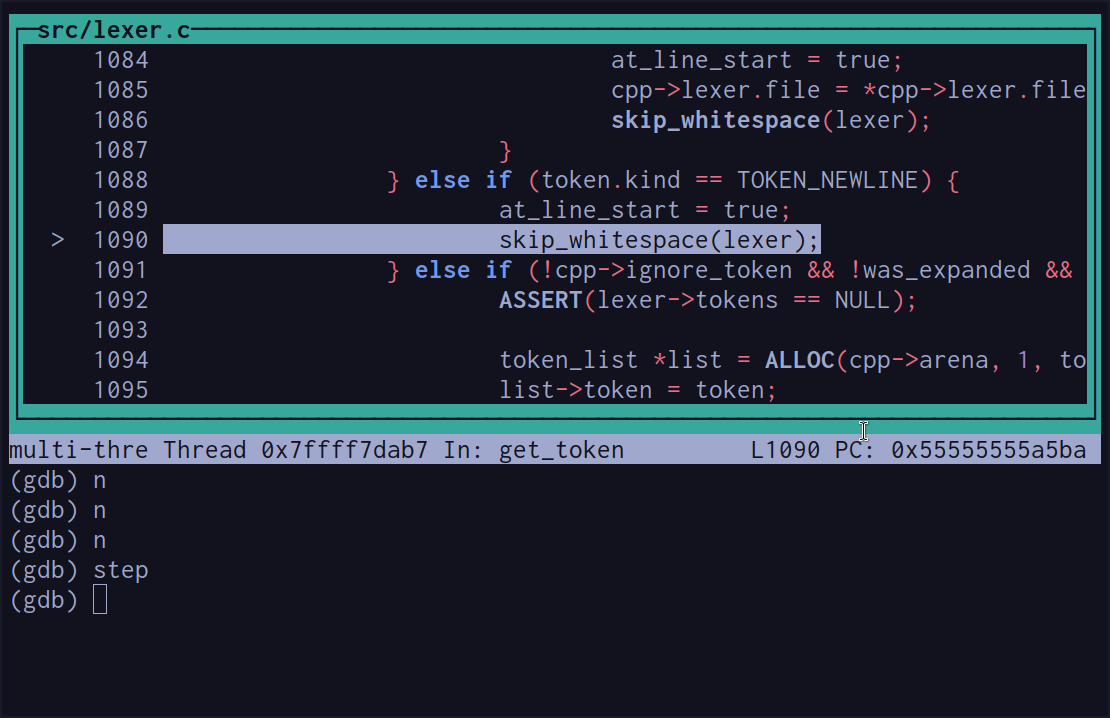
\includegraphics[width=\textwidth]{step.png}
\end{frame}

\begin{frame}
    \todo[inline]{Brief overview of SGX enclaves or just transition to the outline?}
\end{frame}
\fi

\begin{frame}
    \frametitle{Outline}
    \begin{enumerate}
        \item Implementation: SGX-Step
        \item Use case: CopyCat
        \item Mitigation: AEX-Notify
    \end{enumerate}
\end{frame}

\begin{frame}
    \frametitle{SGX-Step}

    \textbf{Goal}: Single-step the execution of an SGX enclave.

    \begin{itemize}
        \item Interrupt enclave after each instruction using APIC timer
    \end{itemize}
    
    \begin{center}
        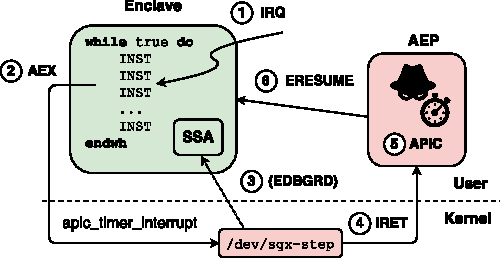
\includegraphics{sgx-step-overview.pdf}
    \end{center}
    {\tiny\hfill\color{gray} Image from \cite{BulckPS17}}
\end{frame}

\begin{frame}{SGX-Step}
    \begin{itemize}
        \item \textbf{Problem}: How long should the timer be?
        \item Too long and we execute multiple instructions (multi-step)
        \item Too short and we're still in \texttt{ERESUME} (zero-step)
    \end{itemize}
\end{frame}

\begin{frame}
    \frametitle{SGX-Step}

    \textbf{Solution}: Induce page faults to increase the latency

    \begin{center}
        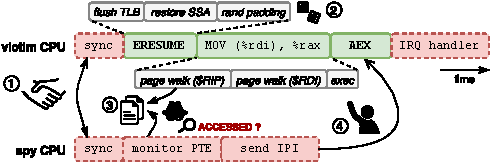
\includegraphics[scale=1.2]{sgx-step-pte.pdf}
    \end{center}

    {\tiny\hfill\color{gray} Image from \cite{ConstableBCXXAK23}}
\end{frame}

\begin{frame}{CopyCat}

    \begin{columns}
        \column{0.2\textwidth}
        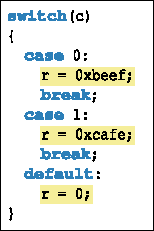
\includegraphics[]{copy-cat-switch-example-only-code.pdf}
        {\tiny\color{gray}Image from \cite{MoghimiBHPS20}}
        
        \column{0.7\textwidth}
        \begin{itemize}
            \item Uses SGX-Step for extracting control-flow
            \item For \emph{inter}-page control-flow: \\ $\Rightarrow$ Track accessed pages in each step
            \item How can we track \emph{intra}-page control-flow?
        \end{itemize}
    
    \end{columns}
\end{frame}

\begin{frame}
    \frametitle{CopyCat}

    \begin{center}
        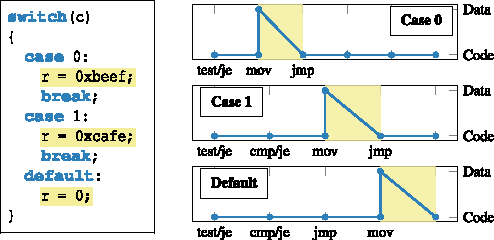
\includegraphics{copy-cat-switch-example.pdf}
    \end{center}

    {\hfill\tiny\color{gray}Image from \cite{MoghimiBHPS20}}
    
    \textbf{Solution}: Compare code and data access patterns with binary
\end{frame}

\begin{frame}{AEX-Notify}
    \begin{itemize}
        \item SGX-Step works because page walk is slow
        \item Large time window where interrupt can land
        \item<2> \textbf{Solution}: Reduce latency by prefetching
    \end{itemize}

    \begin{center}
    \alt<2>
        {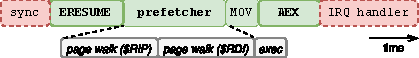
\includegraphics[scale=1.5]{sgx-step-with-prefetch.pdf}}
        {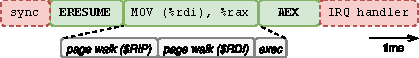
\includegraphics[scale=1.5]{sgx-step-without-prefetch.pdf}}
    \end{center}
    {\tiny\hfill\color{gray} Image from \cite{ConstableBCXXAK23}}
\end{frame}

\begin{frame}{Project Goals}
    \begin{itemize}
        \item Implement single-stepping attack against toy target
        \item Show effectiveness of the attack
        \item Apply the AEX-Notify countermeasure and evaluate its effectiveness
    \end{itemize}
    \textbf{Question}: Is it possible to gather control-flow information with AEX-Notify enabled?
\end{frame}

\begin{frame}[allowframebreaks]{References}
    \bibliography{references.bib}
    \bibliographystyle{alpha}
\end{frame}

\end{document}
